\section{Experimental Results} \label{sec:exp}
\subsection{Experimental Setup}
\label{subsec:experimental-setup}
This experimental section first evaluates the effectiveness of our customized RAG framework for NL2SVA. 
To provide a comprehensive evaluation, we test  it across three LLMs: \textit{OpenAI GPT-4o-mini}, \textit{OpenAI CodeX} which has been fine-tuned on high-quality public code repositories, and \textit{DeepSeek-V3}.
We then evaluate the lightweight \textit{Qwen2.5-Coder-7B-Instruct} model fine-tuned on our synthetic prompt-guided dataset, comparing its performance with the base Qwen model.
We also apply our customized RAG techniques to Qwen and its fine-tuned variants and evaluate their performances.
For methods employing RAG, we retrieve relevant context from the database, which is constructed using $10$ hardware design and verification textbooks.

All experiments are conducted using our evaluation dataset. 
This dataset is the ground truth for evaluating the LLM-generated SVAs in terms of both syntax correctness and functionality match with the natural language property description. 
Two metrics are adopted during evaluation.
\begin{itemize}
    \item \textit{Syntax Correctness (SC)}: number of assertions that are syntactically correct.
    \item \textit{Functionality Match (FM)}: number of assertions that are functionally equivalent to the golden assertions in the evaluation dataset.
\end{itemize}
The two metrics are both derived by the FPV tool \textit{Cadence JasperGold} during our evaluation.
For SC, the FPV tool can directly check the syntax correctness of the LLM-generated SVAs.
For FM, we create the checking SVA by combining the property expression in the golden SVA with that in the LLM-generated SVA using SVA operator \texttt{iff}, as follows:
\begin{verbatim}
     assert property(gold_property_expression 
     iff LLM_property_expression);
\end{verbatim}
If the FPV tool cannot detect any counterexamples for the checking SVA, the two SVAs are functionally equivalent.

Given that our customized RAG framework has multiple components, we perform detailed evaluations on each of them. Specifically, Section~\ref{subsec:exp-evaluation-dynamic} evaluates the effectiveness of the dynamic splitting technique for database construction. 
Section~\ref{subsec:exp-evaluation-hybridretrieval} evaluates the proposed HybridRetrieval method for improving retrieval quality. 
Section~\ref{subsec:exp-evaluate-RAGSVAG} presents an overall evaluation of the customized RAG framework and a comparison with related works.
Finally, Section~\ref{subsec:evaluate-lightweight-llm} evaluates the lightweight Qwen2.5-Coder-7B-Instruct model and its fine-tuned variants using our synthetic dataset, both standalone and integrated with the techniques of our customized RAG framework.

% To assess the effectiveness of the proposed RAG framework, we evaluate both the static splitting technique (\textit{StaticRAG}) and the dynamic splitting technique (\textit{DynamicRAG}) on the prompt-based assertion generation task using our evaluation dataset. 
% To demonstrate the versatility of our framework across different LLMs, we evaluate \textit{OpenAI GPT-4o-mini}, \textit{OpenAI CodeX} which has been fine-tuned on high-quality public code repositories, and \textit{DeepSeek-V3 }, comparing their performance on the assertion generation task. 
% The evaluation is conducted following the automatic framework presented in Fig.~\ref{fig:prompt-assertion-generation-framework}, utilizing Cadence JasperGold~\cite{cadencejaspergold} as the FPV tool to validate both syntax and functionality.
% We use the initial prompt for all methods without using RAG, wile we use the combined prompt for all RAG methods.

% The performance of LLM-generated assertions is measured using the following three metrics:
% \begin{itemize}
%     \item \textit{\#SC} (Syntax Correctness): The number of assertions that are syntactically valid.
%     % \item \#FM (Functionality Correctness): The number of assertions that pass formal verification, meaning no counterexamples exist that violate the assertion.
%     \item \textit{\#FM} (Functionality Match): The number of assertions that are functionally equivalent to the corresponding golden assertions in the dataset.
% \end{itemize}
% Additionally, we evaluate \textit{nl2spec}~\cite{Cosler23}, a related work that employs prompt engineering techniques to improve an LLM’s ability to convert natural language descriptions into temporal logic formulations, which is closely related to SVAs. 
% We modify the prompt of \textit{nl2spec} to be adapted to the SVA generation.
% By including \textit{nl2spec} in our evaluation, we provide a comparative analysis to determine how effective prompt engineering techniques are in enhancing assertion generation accuracy compared to our RAG-aided approach.

\subsection{Evaluation of Dynamic Splitting Technique}
\label{subsec:exp-evaluation-dynamic}
In this subsection, we evaluate the effectiveness of the proposed dynamic splitting technique. 
We compare three methods: applying the base LLM without any retrieval augmentation (\textit{LLM}), applying retrieval augmentation with a database constructed via traditional static splitting (\textit{StaticRAG}), and applying retrieval augmentation with a database constructed using our dynamic splitting  (\textit{DynamicRAG}). 

The evaluation results are summarized in Fig.~\ref{fig:eval-dynamic-splitting}, where the improvement ratio over the basic LLM is shown. 
For GPT-4o-mini, DynamicRAG significantly improves FM by $18.8\%$ compared to LLM, while StaticRAG provides no improvement. 
In terms of SC, DynamicRAG result in $13.5\%$ improvement while StaticRAG only achieves a $2.2\%$ improvement.
When using CodeX, a similar trend is observed. DynamicRAG improves FM by $29.1\%$ over LLM, outperforming StaticRAG ($21.8\%$). 
However, both DynamicRAG and StaticRAG just achieve a slight improvement on SC over LLM.
% SC remains relatively stable across different methods, again suggesting that retrieval augmentation mainly enhances the functional fidelity of generated SVAs.
For DeepSeek, DynamicRAG and StaticRAG even degrade the performance of FM and SC slightly compared to the basic LLM. 
This behavior may be due to DeepSeek’s strong built-in semantic understanding, making it less sensitive to retrieval augmentation quality.
Overall, these results demonstrate that dynamic splitting substantially can help improve the performance of SVA generation for the basic RAG framework.
\begin{figure}
    \centering
    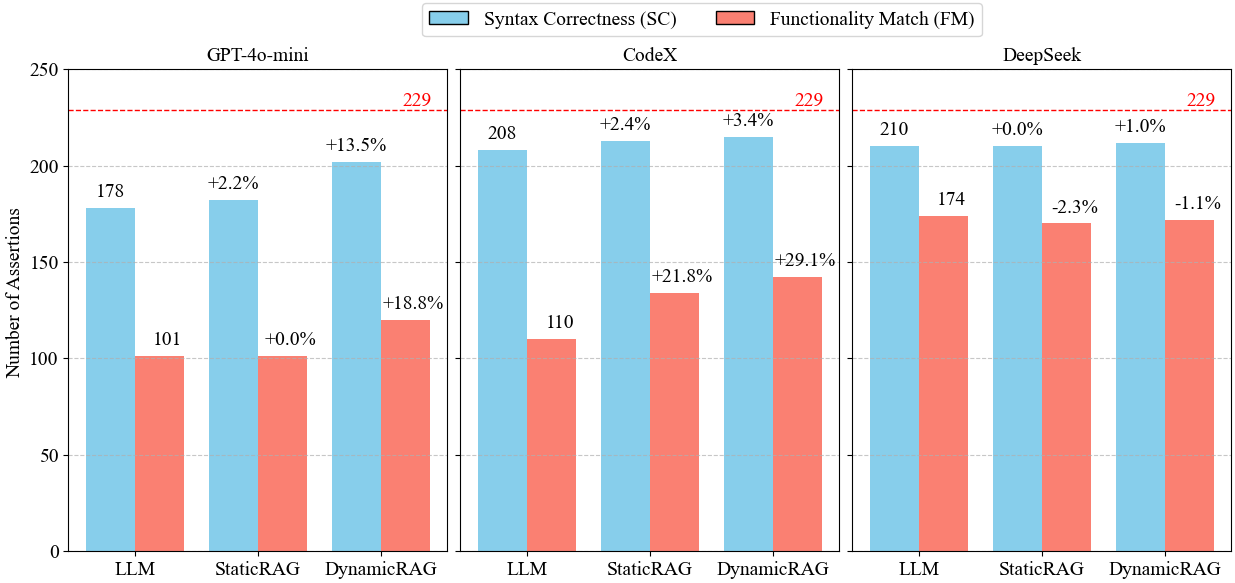
\includegraphics[width=\linewidth]{Figs/exp1_update.png}
    \caption{Evaluation of dynamic splitting technique.}
    \label{fig:eval-dynamic-splitting}
\end{figure}

\subsection{Evaluation of HybridRetrieval}
\label{subsec:exp-evaluation-hybridretrieval}
In this subsection, we evaluate the effectiveness of the proposed HybridRetrieval method. 
Recall that HybridRetrieval consists of the global semantic retrieval and keyword-guided retrieval.
Thus, we compare four methods: (1) using the basic LLM without retrieval augmentation (\textit{LLM}), (2) only global semantic retrieval (\textit{HR-P0}), (3) only keyword-guided retrieval (\textit{HR-P1}), and (4) the full HybridRetrieval (\textit{HR}). In all experiments, the dynamic splitting technique is applied to construct the retrieval database.

The evaluation results are shown in Fig.~\ref{fig:Evaluation-HybridRetrieval}. 
When using GPT-4o-mini, applying HybridRetrieval (both HR-P0 and HR-P1 individually) improves FM substantially compared to the basic LLM. Specifically, HR-P0 improves FM by $18.8\%$ and HR-P1 improves it by $32.7\%$. 
Combining both techniques in HR maintains the $32.7\%$ improvement in FM.
For CodeX, similar trends are observed. HR-P0 and HR-P1 individually improve FM by $18.2\%$ and $19.1\%$, respectively, over the baseline, while the full HybridRetrieval (HR) achieves a $25.5\%$ improvement. 
When evaluating on DeepSeek, improvements are smaller due to the model's stronger built-in understanding ability.  HR still provides consistent FM improvements ($1.1\%$) compared to the baseline, while global semantic retrieval (HR-P0) shows slight $1.1\%$ FM reduction and keyword-guided retrieval (HR-P1) improves by $0.6\%$. 
The full HR yields the best FM performance.

\begin{figure}
    \centering
    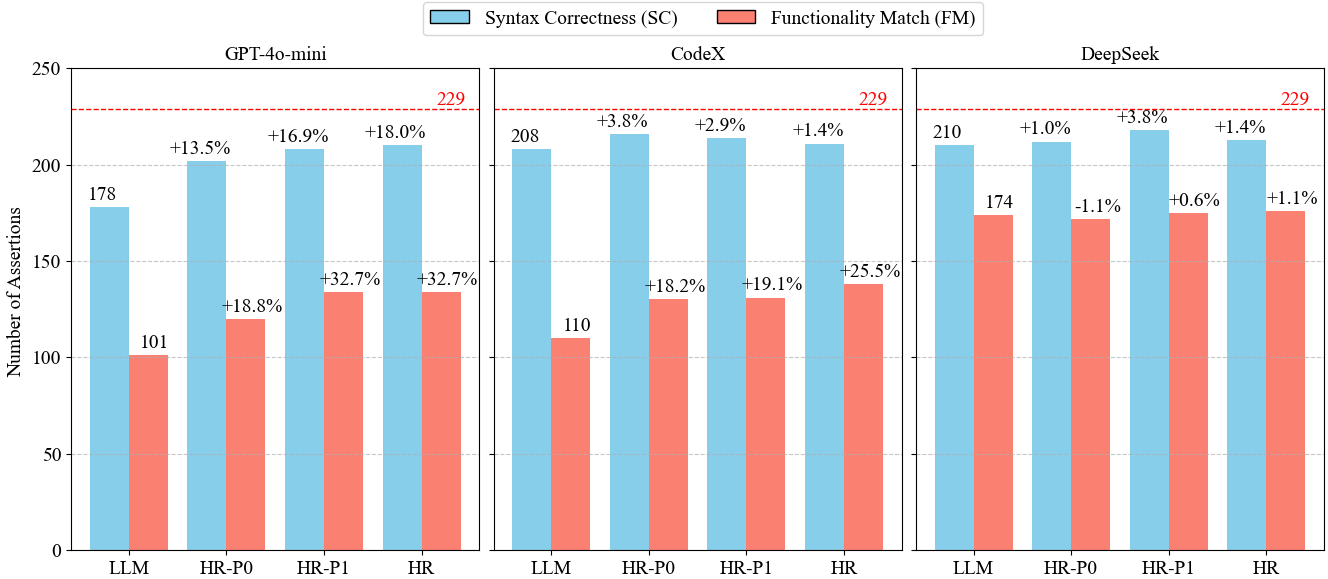
\includegraphics[width=\linewidth]{Figs/exp2_update.png}
    \caption{Evaluation of HybridRetrieval.}
    \label{fig:Evaluation-HybridRetrieval}
\end{figure}

\subsection{Evaluation and Comparison of Customized RAG Framework}
In this subsection, we present the overall evaluation of our full customized RAG framework (\textit{RAGSVAG}) using both HybridRetrieval and SVA operator-based rechecking. Specifically, we do comparison over: applying the plain LLM without any retrieval or augmentation (\textit{LLM}), applying our SVA operator-based rechecking flow without retrieval augmentation (\textit{SOR}), and applying the full RAGSVAG framework. 
For all methods involving RAG, our dynamic splitting technique and HybridRetrieval are employed.
Additionally, we compare our RAGSVAG with \textit{nl2spec}~\cite{Cosler23} and \textit{Spec2Assertion}~\cite{wu2025}.

The results are shown in Fig.~\ref{fig:evaluation-RAGSVAG}. 
Across all the three tested LLMs, RAGSVAG consistently achieves the highest FM among all compared methods, while maintaining competitive SC.
For GPT-4o-mini, applying nl2spec improves FM by $8.9\%$ and applying Spec2Assertion improves FM by $6.9\%$, while SOR alone improves it by $30.7\%$. In contrast, RAGSVAG achieves a FM improvement of $58.4\%$, representing a substantial gain over both baseline and intermediate methods.
For CodeX, similar trends are observed. 
Applying nl2spec improves FM by $18.2\%$ and applying Spec2Assertion improves FM by $25.5\%$, and SOR improves it by $20.0\%$. RAGSVAG can achieve a $34.5\%$ improvement over FM,  outperforming the baselines.
For DeepSeek, which shows strong baseline performance, relative improvements are smaller.  RAGSVAG still achieves a FM improvement of $10.9\%$ compared to the basic LLM, while SOR provide smaller gains, and the nl2spec and Spec2Assertion actually underperform relative to the baseline.
In terms of SC, all methods show smaller improvement, indicating that retrieval and rechecking enhance the FC accuracy of the generated assertions rather than SC.
Overall, the results demonstrate the effectiveness of RAGSVAG in substantially improving the FM of LLM-generated SVAs.

\label{subsec:exp-evaluate-RAGSVAG}
\begin{figure}
    \centering
    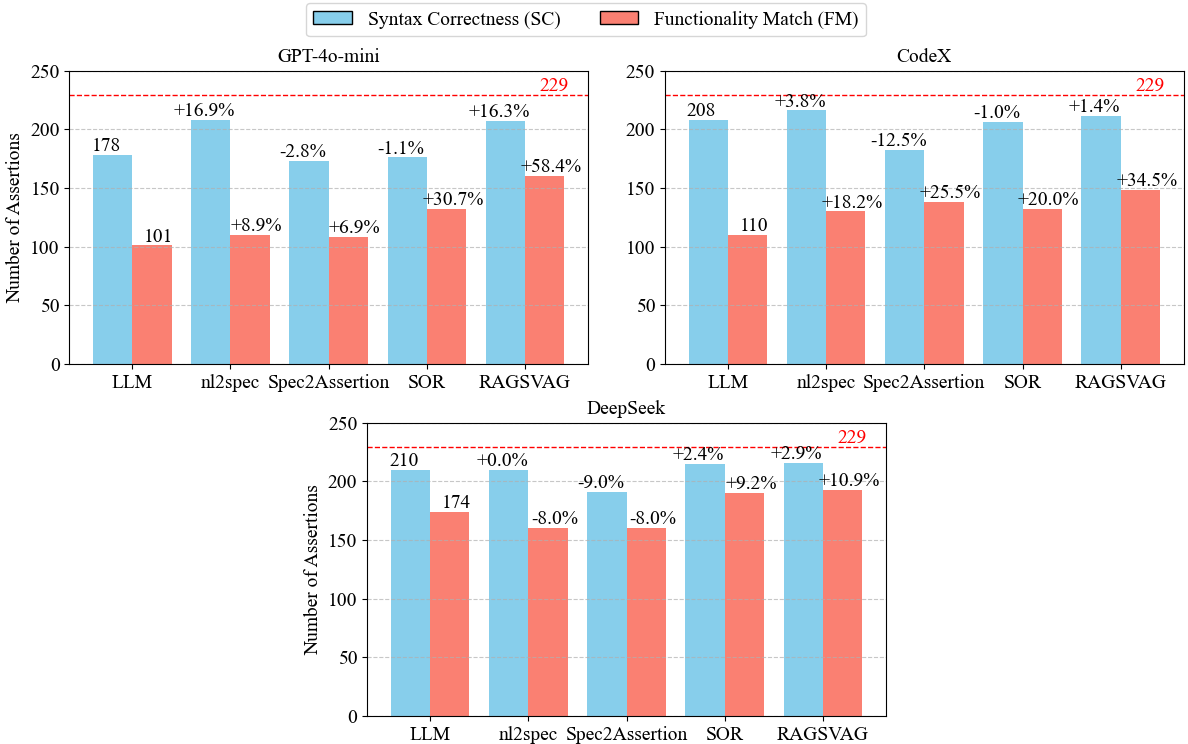
\includegraphics[width=\linewidth]{Figs/exp3_update_1.png}
    \caption{Evaluation and comparison of Customized RAG Framework.}
    \label{fig:evaluation-RAGSVAG}
\end{figure}

\subsection{Evaluation of Finetuned Lightweight LLM}
\label{subsec:evaluate-lightweight-llm}
We evaluate the lightweight \textit{Qwen2.5-Coder-7B-Instruct} model~\cite{hui24} and two fine-tuned variants derived from our synthetic finetuning Dataset in Section~\ref{subsec:synthetic-finetuning-dataset}.  
The first variant, \textit{Qwen-Finetune}, is trained on plain (\emph{SVA, explanation}) pairs from our finetuning dataset following~\cite{Shahidzadeh24}.  
The second, \textit{Qwen-Prompt-Finetune}, is trained on (\emph{SVA, prompt-guided explanation}) pairs.  
The two fine-tuning tasks use supervised learning with \textit{Llama-Factory} \cite{zheng2024llamafactory}, a cosine learning-rate schedule, an initial rate of $8\times10^{-5}$, \texttt{bf16} precision and three epochs.  
Training the two variants on $8 \times$ A100 GPUs requires roughly two hours.

We integrate the techniques from our customised RAG framework into the base Qwen model and its two fine-tuned variants. 
We employ Qwen and its fine-tuned variants with a temperature of $0.6$, top\_p of $0.95$. Considering the format of our fine-tuning dataset and Qwen’s limited context window, we  feed the assertion specification together with the related signals and their natural language explanations, rather than the full Verilog code, into the model or RAG pipeline.

Table \ref{tab:qwen_results} reports results of SC and FM, the corresponding percentages relative to all $229$ SVAs, and the improvements achieved with respect to the base model.
The first column reports the results of the base Qwen. 
The model produces $161$ SC and $105$ FM SVAs, or $70.31 \%$ and $45.85 \%$ of the $229$ SVAs. 
Integrating HybridRetrieval  improves the two metrics to $198$ / $113$. 
Integrating our SVA operator-based rechecking achieves higher SC to $201$ but decreases FM to $101$, and integrating our customized RAG framework ends at $195$ / $101$. 
In short, the base model achieves similar SVA generation performance to that of GPT-4o-mini and benefits from HybridRetrieval, while the SVA operator-based rechecking components help improve SC.

The second column reports the results of Qwen-Finetune. This variant falls to $160$ / $87$, losing $0.62 \%$ in SC and $17.14 \%$ in FM compared with the base model, so we do not integrated any techniques into it. 
By contrast, the third column Qwen-Prompt-Finetune improves SC / FM to $206$ / $148$ ($89.96 \%$ / $64.63 \%$), a $27.95 \%$ SC gain and a $40.95 \%$ FM gain over the base model. 
When HybridRetrieval is integrated, the two metrics continue to be improved to $213$ / $167$, and they remain well above the baseline integrating SVA operator-based rechecking and the overall customized RAG framework. 
These results confirm that fine-tuning the lightweight Qwen model with prompt-guided explanations markedly improves SVA generation, and that integrating the HybridRetrieval component of our customized RAG framework provides an additional improvement.
\begin{table}[t]
\centering
\caption{Evaluation results of the base Qwen model, its finetuned variant, and its prompt-finetuned variant, each used together with our customised RAG framework.}
\label{tab:qwen_results}
% \newcommand{\tabincell}[2]{\begin{tabular}[c]{@{}#1@{}}#2\end{tabular}}
\setlength{\tabcolsep}{1.5pt}
\renewcommand{\arraystretch}{1.35}
\begin{tabular}{@{}lcc cc cc@{}}
\toprule
\multirow{2}{*}{Methods} &
\multicolumn{2}{c}{Qwen} &
\multicolumn{2}{c}{Finetune-Qwen} &
\multicolumn{2}{c}{Prompt-Finetune-Qwen} \\ \cmidrule(lr){2-3}\cmidrule(lr){4-5}\cmidrule(l){6-7}
 & SC & FM & SC & FM & SC & FM \\ \midrule
LLM     & \tabincell{c}{161\\(70.31\%)} & \tabincell{c}{105\\(45.85\%)} & \tabincell{c}{160\\(69.87\%)} & \tabincell{c}{87\\(37.99\%)}  & \tabincell{c}{206\\(89.96\%)} & \tabincell{c}{148\\(64.63\%)} \\
\textit{Improv.} & --- & --- & -0.62\% & -17.14\% & +27.95\% & +40.95\% \\[1ex]
\hline
HR      & \tabincell{c}{198\\(86.46\%)} & \tabincell{c}{113\\(49.34\%)} & --- & --- & \tabincell{c}{\textbf{213}\\(\textbf{93.01\%})} & \tabincell{c}{\textbf{167}\\(\textbf{72.93\%})} \\
\textit{Improv.} & +22.98\% & +7.62\% & --- & --- & \textbf{+32.30}\% & \textbf{+59.05}\% \\[1ex]
\hline
SOR     & \tabincell{c}{201\\(87.77\%)} & \tabincell{c}{101\\(44.10\%)} & --- & --- & \tabincell{c}{208\\(90.83\%)} & \tabincell{c}{155\\(67.69\%)} \\
\textit{Improv.} & +24.84\% & -3.81\% & --- & --- & +29.19\% & +47.62\% \\[1ex]
\hline
RAGSVAG & \tabincell{c}{195\\(85.15\%)} & \tabincell{c}{101\\(44.10\%)} & --- & --- & \tabincell{c}{211\\(92.14\%)} & \tabincell{c}{164\\(71.62\%)} \\
\textit{Improv.} & +21.12\% & -3.81\% & --- & --- & +31.06\% & +56.19\% \\ \bottomrule
\end{tabular}
\end{table}


% Fig.~\ref{fig:GPT-4o-mini} and~\ref{fig:GPT-4o} present comparative experimental results of different methods using \textit{GPT-4o-mini} and \textit{CodeX}, respectively. 
% We evaluate these methods based on the three critical metrics \#SC, \#FM, and \#FM.

% As depicted in Fig.~\ref{fig:GPT-4o-mini}, using \textit{GPT-4o-mini} as the baseline, we observe that the \textit{nl2spec} method significantly enhances performance, achieving a $16.9\%$ improvement in \#SC, along with notable gains in \#FM ($7.8\%$) and \#FM ($8.9\%$). 
% The \textit{StaticRAG} method, however, yields only marginal improvement ($2.2\%$) in \#SC, with no observable change in \#FM and \#FM. 
% In contrast, the \textit{DynamicRAG} method demonstrates substantial performance enhancements across all metrics, achieving improvements of $13.5\%$ in \#SC, $18.6\%$ in \#FM, and $18.8\%$ in \#FM, clearly highlighting its effectiveness over \textit{StaticRAG}.

% In Fig.~\ref{fig:GPT-4o}, it shows similar experiments conducted with \textit{CodeX} as the baseline model. 
% Here, the \textit{nl2spec} method moderately increases \#SC by $3.8\%$, and significantly boosts \#FM and \#FM by $18.0\%$ and $18.2\%$, respectively. 
% \textit{StaticRAG} achieves comparable but slightly lower gains in \#SC ($2.4\%$), but substantially higher improvements in \#FM and \#FM ($21.6\%$ and $21.8\%$, respectively). 
% The \textit{DynamicRAG} method surpasses all other approaches, delivering the highest improvements observed: $3.4\%$ in \#SC, $28.8\%$ in \#FM, and $29.1\%$ in \#FM. 
% These results underscore \textit{DynamicRAG}'s consistent advantage, showing its ability to notably enhance the capabilities of \textit{CodeX}.

% Overall, the experimental analysis clearly indicates that augmenting the two baseline LLMs with the \textit{DynamicRAG} method consistently delivers better performance across all measured criteria, proving its practical effectiveness for improving LLM-aided assertion generation.


% \begin{figure}
%     \centering
%     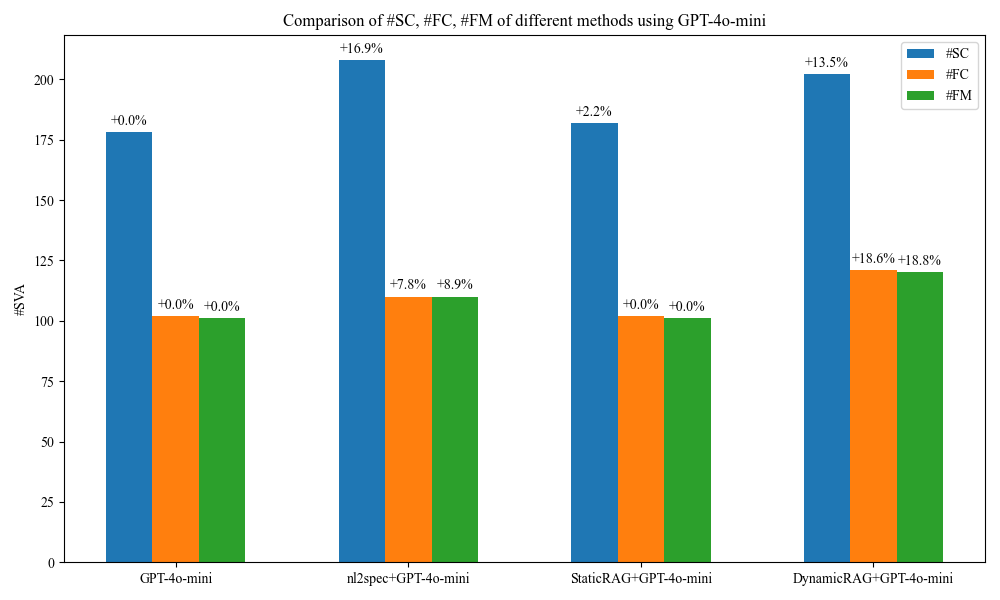
\includegraphics[width=\linewidth]{Figs/Figure_1.png}
%     \caption{Comparison of \#SC, \#FM, \#FM of different methods using \textit{GPT-4o-mini}.}
%     \label{fig:GPT-4o-mini}
% \end{figure}

% \begin{figure}
%     \centering
%     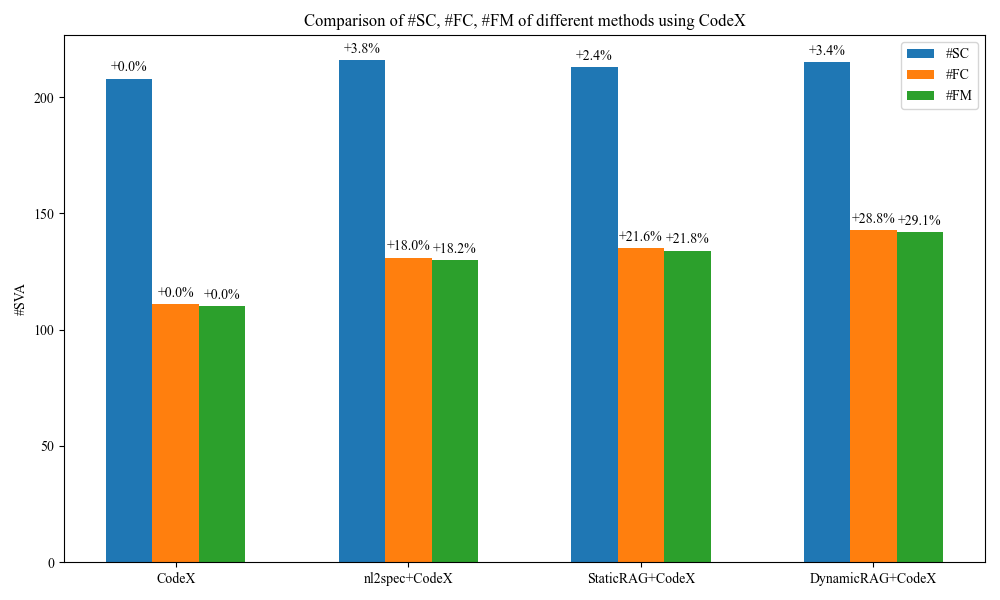
\includegraphics[width=\linewidth]{Figs/Figure_2.png}
%     \caption{Comparison of \#SC, \#FM, \#FM of different methods using \textit{CodeX}.}
%     \label{fig:GPT-4o}
% \end{figure}

% \subsection{Example SVAs Generated by RAGSVAG}
% \label{subsec:exp-example-svas}
% To  illustrate the effectiveness of RAGSVAG, we select $10$ natural language property explanations from our evaluation dataset. 
% For each explanation, we show the corresponding SVAs generated by the baseline GPT-4o-mini and by RAGSVAG, as summarized in Table~\ref{tab:example_svas}. 
% In addition, we provide the  design name and the number of lines in the Verilog code for each example, offering more context about the complexity of the design where the property originates.

% Each generated assertion is further validated using the proposed assertion verification framework described in Section~\ref{subsec:Evaluation-Dataset}. Specifically, we check whether the generated SVA correctly matches the intended functionality described in the natural language property.
% Across all $10$ examples, the SVAs generated by RAGSVAG pass the functionality verification, meaning they accurately implement the property. In contrast, the SVAs generated by GPT-4o-mini exhibit functionality mismatches in every case.  Common issues include incorrect usage of temporal operators (such as overlapping implication operator \texttt{|->} and non-overlapping implications operator \texttt{|=>}), improper handling of past signal values, and failure to accurately capture the specified clock-cycle timing relationships.

% % \begin{table*}[ht]
% %     \centering
% %     \caption{Examples of SVAs generated by GPT-4o-mini and RAGSVAG.}
% %     \label{tab:example_svas}
% %     \begin{tabular}{|c|c|p{3.8cm}|p{5.4cm}|p{5.4cm}|}
% %         \hline
% %         \textbf{Design} & \textbf{Lines} & \textbf{Natural Language Property} & \textbf{GPT-4o-mini SVA} & \textbf{RAGSVAGen SVA} \\
% %         \hline
% %         ff & $10$ & When enable signal is set (1), output equals input from previous cycle in next cycle. & \texttt{assert property (@(posedge clk) disable iff (rst) (en == 1'b1 |=> out == in[1]));} & \texttt{assert property (@(posedge clk) disable iff (rst) (en |=> (out == \$past(in))));} \\
% %         \hline
% %         pwm & $18$ & Eventually, the inversion of the output becomes true. & \texttt{assert property (@(posedge clk) (s\_eventually (!pulse)));} & \texttt{assert property (@(posedge clk) (pulse |-> eventually (!pulse)));} \\
% %         \hline
% %         register & $20$ & When enable reset (0), output equals last output in next cycle. & \texttt{assert property (@(posedge clk) disable iff (rst) (en == 0 |-> out == out[1]));} & \texttt{assert property (@(posedge clk) disable iff (rst) (en == 0 |=> (out == \$past(out))));} \\
% %         \hline
% %         simple\_req\_ack & $31$ & When request signal is detected to have a rising edge, then after a delay of $2$ clock cycles the acknowledge signal is detected to have a rising edge. & \texttt{assert property (@(posedge clk) disable iff(!rst\_n) (req\_ff in \{1'b0, 1'b1\} during [2] |=> (ack\_ff == 1'b1)));} & \texttt{assert property (@(posedge clk) disable iff(!rst\_n) (\$rose(req) |=> \#\#2 \$rose(ack)));} \\
% %         \hline
% %         or1200\_if & $194$ & When pipeline flush signal is reset ($0$) and save instruction condition is true, then saved flag equals 1 in the next clock cycle. & \texttt{assert property (@(posedge clk) disable iff (rst) (if\_flushpipe == 0 \&\& save\_insn |-> saved));} & \texttt{assert property (@(posedge clk) disable iff (rst) (if\_flushpipe == 0 \&\& save\_insn |=> (saved == 1)));} \\
% %         \hline
% %         arbiter & $231$ & When the first bit of grant output is asserted and in the previous clock cycle the arbitration type selector signal was equal to $0$, then the first bit of request input signal from the previous clock cycle must be asserted in the current clock cycle. & \texttt{assert property (@(posedge clk) disable iff (\textasciitilde rst\_n) (gnt[0] \&\& arb\_type == 0 |-> req[0]));} & \texttt{assert property (@(posedge clk) disable iff (\textasciitilde rst\_n) ((gnt[0] \&\& \$past(arb\_type) == 0) |-> \$past(req[0])));} \\
% %         \hline
% %         a25\_wishbone & $447$ & When the wishbone bus state equals \texttt{WB\_BURST1} and the acknowledgement signal is asserted, then the wishbone bus state equals \texttt{WB\_BURST2} in the next clock cycle. & \texttt{assert property (@(posedge i\_clk) (wishbone\_st == WB\_BURST1 \&\& i\_wb\_ack |-> (wishbone\_st == WB\_BURST2)));} & \texttt{assert property (@(posedge i\_clk) ((wishbone\_st == WB\_BURST1 \&\& i\_wb\_ack) |=> (wishbone\_st == WB\_BURST2)));} \\
% %         \hline
% %         control\_unit & $602$ & When the signal that indicates the beginning of an AES operation equals 0, then the signal used to initialize the key generation process equals 0 in the current clock cycle. & \texttt{assert property (@(posedge clk) (start == 0 |=> key\_init == 0));} & \texttt{assert property (@(posedge clk) (start == 1'b0 |-> key\_init == 1'b0));} \\
% %         \hline
% %         or1200\_ctrl & $1225$ & When the freeze signal for the EX stage is reset ($0$) and either the freeze signal for the ID stage is set ($1$) or the pipeline flush signal for the EX stage is set ($1$), then the signal indicating a MAC read operation in the EX stage equals 0 in the next clock cycle. & \texttt{assert property (@(posedge clk) disable iff (rst) (!ex\_freeze \&\& (id\_freeze || ex\_flushpipe) |-> (ex\_macrc\_op == 0)));} & \texttt{assert property (@(posedge clk) disable iff (rst) ((!ex\_freeze \&\& (id\_freeze || ex\_flushpipe)) |=> (ex\_mac\_op == 0)));} \\
% %         \hline
% %         module\_i2c & $3382$ & When the FIFO receiver empty indicator equals $1$, then the FIFO receiver empty output equals $1$ in the current clock cycle. & \texttt{assert property (@(posedge PCLK) (fifo\_rx\_f\_empty == 1'b1 |-> fifo\_rx\_wr\_en == 1'b1));} & \texttt{assert property (@(posedge PCLK) (fifo\_rx\_f\_empty == 1'b1 |-> RX\_EMPTY == 1'b1));} \\
% %         \hline
% %     \end{tabular}
% % \end{table*}

% % \subsection{Evaluation Results over CodeLlama}
% % \label{subsec:results-over-CodeLlama}
% % In Fig.~\ref{fig:CodeLlama}, it illustrates the performance of augmentation methods with \textit{CodeLlama} as the baseline. 
% % \textit{CodeLlama} initially demonstrates considerably poorer performance compared to \textit{OpenAI} models across all metrics. 
% % To mitigate this, prompts are augmented with used signals for each golden assertion, represented by lighter-colored portions of each bar, which reflect the quantitative improvements after adding signals into the prompt. 
% % Note that the used signals can be directly extracted from our evaluation dataset.
% % Notably, the \textit{StaticRAG} method with signals slightly improves \#SC by $0.5\%$, while achieving meaningful gains in \#FM ($5.0\%$) and \#FM ($5.1\%$). 
% % The \textit{DynamicRAG} method yields a small decrease in \#SC ($-1.5\%$) but provides substantial improvements in \#FM ($8.0\%$) and \#FM ($8.1\%$), indicating the effectiveness of including used signals in enhancing assertion generation. 
% % Thus, identifying relevant signals from Verilog code is crucial for assertion generation and relies heavily on the code explanation capability of an LLM. 
% % \textit{CodeLlama}, however, exhibits limitations in this regard.

